\documentclass[11pt]{article}
\usepackage[margin=0.85in]{geometry}
\usepackage{amsmath,amssymb,graphicx,booktabs,hyperref}
\graphicspath{{./}}
% Editorial revision; scientific execution dates stated below.
\newcommand{\FActualDate}{22 October 2026 revision}
\newcommand{\FProfileFigure}{figures/F_geometry06_v2/profile_meshes.png}
\newcommand{\FDerivativeFigure}{figures/F_geometry06_v2/geometry_and_derivative_steps.png}
\title{F continuation: background nuisance estimation}
\author{}
\date{\FActualDate}
\begin{document}
\maketitle
\noindent This manuscript companion reports a bounded exploratory continuation;
it does not replace the historical results in the paper. Existing credits and
licence scopes remain unchanged. This editorial revision is dated 22 October
2026. Scientific execution occurred on 19 October 2026 UTC (20 October in
New Zealand at completion); no new scientific computation accompanies this
revision.

\section*{Question and four procedures}
The question is whether background nuisance treatment changes a fixed finite
inhibition procedure, and whether conditional likelihood compensation or
numerical stopping sensitivity helps explain the observed differences.
No physical or causal explanation follows merely from a favourable contrast.
All alternatives estimate inhibition $\eta$; the null fixes $\eta=0$.
\begin{center}
\begin{tabular}{lll}\toprule
Cell & Free null coordinates & Free alternative coordinates\\\midrule
$I_{00}$ & none & $\eta$\\
$I_{10}$ & $a$ & $(a,\eta)$\\
$I_{01}$ & $d$ & $(d,\eta)$\\
$I_{11}$ & $(a,d)$ & $(a,d,\eta)$\\\bottomrule
\end{tabular}
\end{center}
Here $a,d$ are background log level and trend; other parameters are supplied
according to the pinned law. Supplied/supplied is not a fixed-$\eta$ oracle.
The original procedure is distinct from the separately labelled solver
and geometry diagnostics.

\section*{Strict marked-history accounting}
For a fixed observed history, write
\[
 \lambda(t)=\exp\{a+d x(t)-\eta G(t)\}+nH(t),\qquad
 \ell=\sum_i\log\lambda(t_i^-)+\sum_i\log f_\beta(q_i)
       -\int_0^T\lambda(t)\,dt .
\]
Here $x(t)=2t/(24394\,\mathrm{days})-1$ is the actual affine
observation coordinate, with $t$ measured in days; it is not $1/t$ or a
Taylor approximation.
Only earlier events enter $G(t_i^-),H(t_i^-)$. The current mark affects later
history, not its own event intensity. Initial quiet and terminal exposure,
all earlier parents and the exact supplied projected/paired clock convention
are retained. No clock or mark repair is introduced.

The direct contrast retains event and complete compensator accounting.
With the same supplied $n$, trigger kernel/productivity and mark law, trigger
exposure and common mark terms cancel between null and alternative. This is
an explicit cancellation, not a reason to omit those terms in comparisons
that change them. Event-log terms cannot be additively allocated to latent
causes. The primary numerical procedure is order 16 with mandatory order-32
and other prescribed controls. A finite candidate does not override an
unresolved optimizer or control status. Bounded recipes establish neither
global optima nor equal effective complexity.

\section*{Conditional amplitude profile}
Fix $d,\eta,n$, kernels, mark law and history, and let
\[
 A=e^a,\quad u_i=e^{d x_i-\eta G_i},\quad v_i=nH_i,\quad
 Q=\int_0^T e^{d x(t)-\eta G(t)}dt,\quad C=n\int_0^TH(t)dt .
\]
The ground negative log likelihood, omitting only the common mark constant,
is $L(A)=AQ-\sum_i\log(Au_i+v_i)+C$. Hence
\[
 L_A=Q-\sum_i\frac{u_i}{Au_i+v_i},\qquad
 L_{AA}=\sum_i\left(\frac{u_i}{Au_i+v_i}\right)^2\geq0 .
\]
Convexity holds in $A$, not generally in $a$. With
$p_i=Au_i/(Au_i+v_i)$, $L_{aa}=AQ-\sum_i p_i(1-p_i)$ can be negative.
The constrained profile uses $A\in[e^{-12},1]$: a nonnegative lower-end
$L_A$ selects the lower boundary; a nonpositive upper-end $L_A$ selects the
upper boundary; otherwise a bracketed scalar root is used. When every
$v_i=0$, $N/Q$ gives the unconstrained stationary point, restricted to the
allowed interval; an empty history selects the lower boundary.

The implementation reports actual derivative/KKT tolerance, amplitude
bracket width, stopping reason and exact/approximate status. Its parameter
named \texttt{a\_tolerance} gates width in $A$, not absolute error in $a$.
Interior acceptance can be curvature/bracket-width limited; it must not be
described as meeting a fixed derivative threshold alone. The conditional
mesh fixes the remaining parameters and is not a confidence region.
The $\eta=0$ analytic background branch and positive-$\eta$ quadrature branch
have a separately recorded numerical seam. All four prescribed difference
steps are retained, with truncation/cancellation and boundary-domain cautions;
no best step repairs a scientific acceptance rule.

\section*{Realized-event geometry}
At a fixed point the event log-intensity columns are
\[
 c_i=(p_i,\;p_i x_i,\;-p_iG_i),\qquad
 Z=W^{1/2}C_{\rm event} .
\]
Main06 uses $W=I_N$, so every actual event weight is one. The factors
$p_i$ already enter the event columns; quadrature weights are separate.
The raw Gram matrix is $Z^\top Z$. Nonzero weighted columns are normalized
by their Euclidean norms before numerical SVD/projection. If $\widetilde z_\eta$
is the scaled inhibition column and $P_{a,d}$ the numerical least-squares
projection on the scaled nuisance columns, the reported residual is
\[
 r_\eta=\frac{\|(I-P_{a,d})\widetilde z_\eta\|_2^2}
                  {\|\widetilde z_\eta\|_2^2} .
\]
This is a \emph{squared} residual fraction, not a norm ratio. A zero
inhibition column is explicitly undefined for interpretation, despite its
reported zero convention. The event Gram excludes compensator derivatives
and random-history variation: it is not a full observed Hessian, ensemble
Fisher information, sampling covariance, global identification theorem or
causal quantity. Low residuals describe conditional path overlap only.

\section*{Completed portions and missing work}
The independently reviewed geometry stage is partial: six of 11 cases
completed, two timed out, one was started-unknown at the tree-RSS stop and
two were unattempted. All 11 remain in accounting and figures. The saved
portion has 253 of 396 solver rows and 840 of 1,540 profile points, with
840 corresponding order-32 controls. Two old failure witnesses were
intentionally selected separately from nine metadata extrema; neither
selection estimates population prevalence or detection probability.

The old witnesses reproduced maxls=40 ABNORMAL returns; diagnostic
maxls=100 returned success at unchanged objective and essentially unchanged
parameters. This is stopping-flag sensitivity, not proof of the precise old
cause, gradient convergence or a corrected production outcome. No old
unresolved status is promoted, and maxls=100 is not substituted into calibration.

The separate ended nine-case full-procedure tail run produced seven complete
cases and 31 of 36 controlled method outcomes. One finite candidate lacked
final controls and four methods were absent; all five remain unknown.
The large alternative case timed out during its Powell control, while the
largest null case failed the unchanged internal 128 MiB feature-cache limit.
An external 2 GiB tree lease did not relax that internal limit or repair the
saved failure. These stress cases do not demonstrate complete bank coverage.

\begin{figure}[p]
\centering\includegraphics[width=\textwidth]{\FProfileFigure}
\caption{All 11 planned geometry cases, including explicit missing panels.
Conditional profile NLL is not a confidence region; colour saturation is
labelled in the reviewed image.}
\end{figure}
\begin{figure}[p]
\centering\includegraphics[width=\textwidth]{\FDerivativeFigure}
\caption{Realized-event overlap and all saved $\eta=0$ derivative steps.
Positive absolute errors use a log display; exact zeros, if any, are listed
separately without floors, clipping or imputation. Selected old witnesses
remain distinct. Neither panel establishes a causal mechanism.}
\end{figure}

\section*{Calibration and uncertainty contract}
Let $R$ be the planned reference count, $K$ the controlled reference indices,
$U=R-|K|$, and $E_q=\sum_{r\in K}\mathbf 1\{T_r\geq T_q\}$ for a controlled
query statistic. The add-one rank interval is
\[
 p_q\in\left[\frac{1+E_q}{R+1},\frac{1+E_q+U}{R+1}\right].
\]
Ties use $\geq$. An uncontrolled query remains unknown. An upper endpoint
at most $\alpha$ gives a definite rejection; a lower endpoint above $\alpha$
gives a definite non-rejection; otherwise the decision remains unknown.
For $N$ planned queries, $k$ definite rejections and $u$ unknowns give
accounting bounds $[k/N,(k+u)/N]$, not sampling confidence intervals.

For the paired nuisance interaction,
\[
 D_i=I_i^{00}-I_i^{10}-I_i^{01}+I_i^{11},\qquad
 \overline D=N^{-1}\sum_iD_i,\qquad
 \operatorname{MCSE}=\sqrt{\frac{\sum_i(D_i-\overline D)^2}{N(N-1)}} .
\]
The declared point summary requires all planned paired rows resolved and
$N\geq2$; it is conditional on the fixed reference bank, not a survivor-only
estimate or reference-bank uncertainty measure.

The executed method used 2,000 shared-reference and paired-query resamples
as a separately gated descriptive sensitivity analysis, not automatic
confirmatory, simultaneous or unconditional coverage. Historical independence
is source-reported, and adaptive pilot/cost-query reuse remains relevant.
Both production jobs ended before final calibration. Independent review
reconstructed base decisions, replayed all 2,000 shared-reference plans and
checked all 80 chunk hashes. It independently recalculated eight declared
query-replicate witnesses.
A separate audit checked all 120 saved endpoint quantiles. This does not mean
every resampled query statistic was independently recalculated.

% Values retained from the independently audited saved-output checkpoint.
\section*{Actual bounded checkpoint}
The final inventory retains 2,149 histories: 999 references, 1,000 null
queries and 150 alternative queries. Of 8,596 planned method outcomes,
7,068 have controlled statistics and 1,528 remain unknown. There are 1,752
histories with all four controlled, 18 partial, three with exceptions and
376 never attempted. One of the partial claimed histories was interrupted with
an uncontrolled final method. Registration is not complete computation.
The two production phases produced 1,639 new terminal records and reused
133 immutable carried records; the claim count was 1,640.

At $\alpha=0.05$, the final accounting is:
\begin{center}
\begin{tabular}{llrrrr}\toprule
Queries & Cell & Reject & Non-reject & Unknown & Rejection bounds\\\midrule
Null ($N=1000$)&$I_{00}$&30&593&377&$[0.030,0.407]$\\
&$I_{10}$&35&588&377&$[0.035,0.412]$\\
&$I_{01}$&31&586&383&$[0.031,0.414]$\\
&$I_{11}$&31&589&380&$[0.031,0.411]$\\\midrule
Alternative ($N=150$)&$I_{00}$&150&0&0&$[1,1]$\\
&$I_{10}$&122&28&0&$[0.8133,0.8133]$\\
&$I_{01}$&150&0&0&$[1,1]$\\
&$I_{11}$&65&82&3&$[0.4333,0.4533]$\\\bottomrule
\end{tabular}
\end{center}
The finite fitting recipe reported here gives 122 rejections out of 150
for $I_{10}$ and 65 rejections, 82 non-rejections and three unknown decisions
for $I_{11}$. These are distinct from the paper's historical counts of
123/150 and 68/150, respectively. A separate source-reported metadata check
matched historical and continuation input identities and case roles; this
compact packet does not reproduce it. No paired historical/continuation
outcome comparison is reported; the counts should not be combined or
interpreted as a paired change in detection.

These are bounds over all planned queries, not confidence intervals or
estimates conditional on successful fitting. Controlled reference counts
are 998, 998, 992 and 997 in cell order; controlled null-query counts are
623, 623, 619 and 620; alternative counts are 150, 150, 150 and 148.
Thus a controlled query can still have an unresolved decision because
reference uncertainty straddles the threshold. Null missingness depends
on history cost, traversal and deadlines; the broad bounds do not establish
empirical 5\% size.

The nuisance-interaction accounting bounds are $[-0.765,0.752]$ under
the null and $[-0.38,-0.36]$ under the alternative. The required full-pair
point mean and MCSE are unavailable for both roles. No survivor-only point
estimate is substituted. On these 150 saved alternative histories, supplying
level and estimating trend gives 150 definite rejections;
estimating both nuisance coordinates is associated with materially fewer
detections. The signed interaction is a procedure contrast, not a causal
effect or proof of physical inhibition.

\subsection*{Completed descriptive resampling}
All 2,000 declared replicates completed, using one shared reference plan
across the four cells and both roles, and separate paired query plans by
role. Lower and upper accounting endpoints are summarized separately with
linear/type-7 quantiles. For the alternative $I_{11}$ cell, the 2.5\%, median
and 97.5\% quantiles of the lower endpoint are $(0.3800,0.4333,0.4667)$
for bank-only resampling and $(0.3400,0.4333,0.5200)$ when paired queries
are also resampled. The corresponding upper-endpoint quantiles are
$(0.4067,0.4533,0.4800)$ and $(0.3600,0.4533,0.5400)$.
These summarize sensitivity of incomplete accounting, not certified coverage.
All 120 endpoint quantiles and counts of every replicate status are retained
in the JSON/CSV tables; individual statuses remain in the saved chunk JSON.
No unresolved replicate is discarded. In the alternative
paired-query mode, 126 replicates have a resolved point interaction and
1,874 remain unresolved. This does not resolve the original full-pair point.

\subsection*{Posthoc accounting of the continuation pilot}
This subsection concerns the earlier 25-query pilot of this continuation,
not the paper's separate $\eta$-planning experiment (6/25 versus 11/25).
After inspecting the aggregate calibration, a separate saved-evidence check
fixed the original 25 alternative IDs and compared their unchanged carried
scores under the old and expanded reference banks. This was descriptive
posthoc accounting: no fit, rank plan or history was regenerated.
For $I_{10}$, the original cohort changed from $(6,11,8)$ to $(19,6,0)$
in reject/non-reject/unknown counts. The remaining 125 alternatives gave
$(103,22,0)$ under the same final bank. For $I_{11}$, the original cohort
changed from $(6,17,2)$ to $(8,17,0)$ and the remaining cohort gave
$(57,65,3)$. Both cohorts have all rejections in $I_{00}$ and $I_{01}$.
The same 25 fitted scores yield different decisions under the new reference
calibration. This comparison does not isolate bank size from reference
composition, rank resolution or missingness. Neither
this comparison nor the additional query cohort establishes population
causality, independent validation or nominal test size.

\begin{figure}[p]
\centering
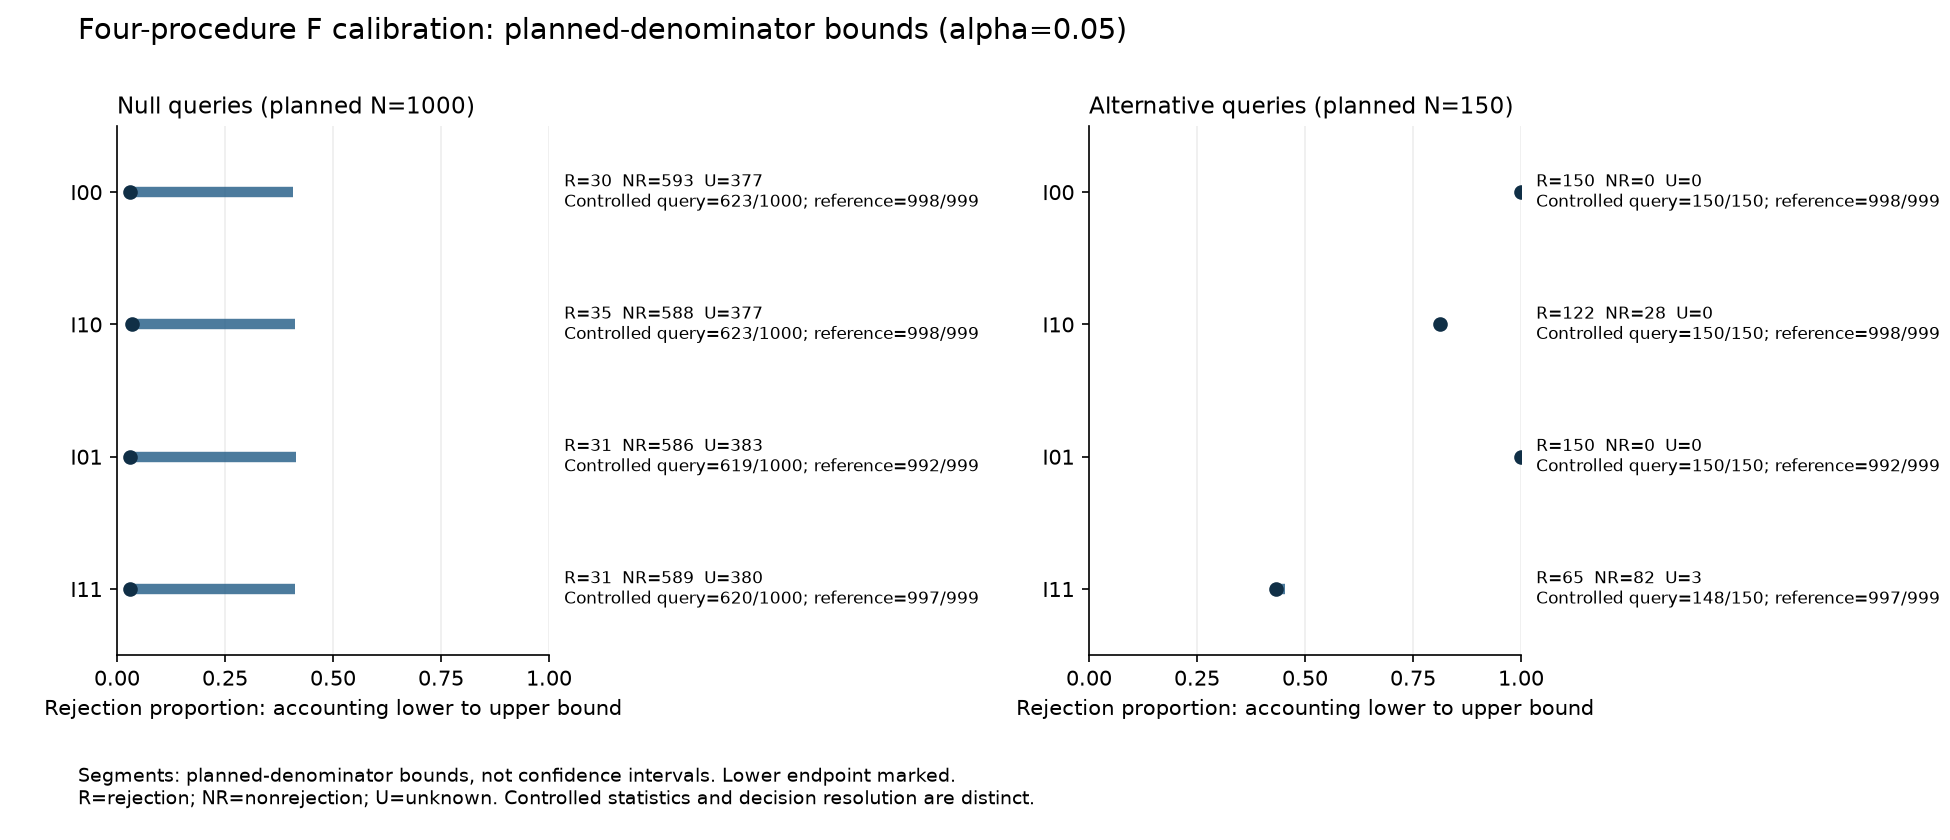
\includegraphics[width=\textwidth]{figures/F04_calibration01/F04_planned_denominator_bounds.png}
\caption{Actual final calibration on the full planned denominators.
Segments span definite rejection through rejection plus unresolved outcomes;
they are accounting bounds. The figure retains unknowns and controlled
query/reference counts.}
\end{figure}

\subsection*{Next decision}
The continuation stops at this incomplete evidence checkpoint. Incomplete
null coverage prevents a calibrated-size conclusion. Reopening the study
would first require a bounded demonstration of a substantially cheaper,
numerically valid recovery procedure, with consistent rules across roles
and cells. Old failures would remain preserved, and any reference-bank
change would require recalibration of the entire contrast. No such recovery,
cache change, fresh bank or wider scientific campaign accompanies this
manuscript revision.


\section*{Availability and bounded interpretation}
The 2,149 reused bank byte/clock identities were reverified; the historical
RNG and generating process were not replayed. The private NPZ bank is not
included in source-only material. Exact excluded inputs, settings and receipts
are required for historical reproduction; constructed fixtures are separate.
The accompanying saved summary, accounting tables and figures document the
reported numerical checkpoint; they do not replace the omitted raw inputs.

Conditional overlap, solver flags and controlled calibration outcomes must be
interpreted together with failures and missing tails. They do not identify
physical inhibition or justify an automatic cache change, retry, new bank,
broader search or next cycle. Any such work remains a separately reviewed
proposal. This companion makes no claims about the other research tracks.
\end{document}
